%
% Capítulo 1
%
\chapter{Introdução} \label{cap1}

Atualmente, são várias as aplicações responsáveis por fornecer listas de compras, porém carecem de controlo de stocks e conhecimento dos hábitos dos seus utilizadores. Neste projeto pretende-se desenvolver uma aplicação que permite a gestão e controlo de stocks de produtos alimentares na despensa de qualquer casa. Os padrões de consumo dos utilizadores são registados, permitindo prever a data da rotura de stock de produtos.

%
% Secção 1.1
%
\section{Abordagem} \label{sec11}

No contexto do projeto assume-se a existência de duas formas de apresentação para os produtos: avulsos e embalados. Os primeiros são conservados em sistemas de arrumação marcados com \textit{tags} programáveis por \textit{smartphones}. Os detalhes dos itens são especificados pelo utilizador e carregados para a \textit{tag}. Enquanto que para os produtos embalados, admite-se que os produtores utilizam \textit{tags}, \acrfull{nfc} ou \acrfull{rfid}, para guardar os rótulos de forma digital e em formato standard.

Após a aquisição, os artigos são armazenados em locais que devem dispor de dispositivos de hardware equipados com leitores de \textit{tags}. É recolhida a informação presente na \textit{tag}, identificado o tipo de movimento (entrada ou saída) e enviado para a \gls{api-web}.

%
% Secção 1.2
%
\section{Metas e Objetivos} \label{sec12}
Têm-se como objetivos, os seguintes pontos:
\begin{itemize} \itemsep 0pt
	\item Desenho e Implementação das Aplicações Móvel e Web
	\item Elaboração do Algoritmo de Previsão de Stocks
\end{itemize}


%
% Secção 1.3
%
\section{Especificações do Projeto e Resumo da Solução} \label{sec13}

\begin{figure}[H]
	\centering
	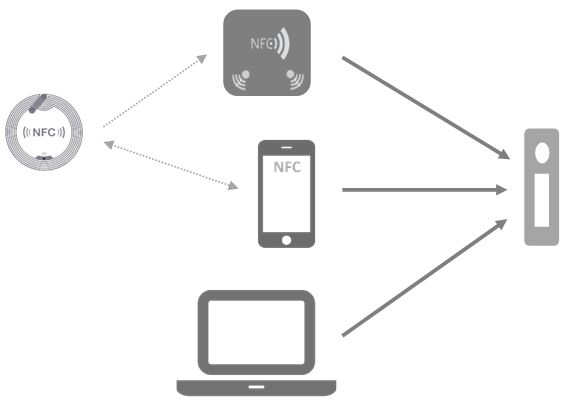
\includegraphics[width=12cm, scale=1]{./figures/project_structures.png}
	\caption{Estrutura do Projeto}
	\label{project-structure}
\end{figure}

\begin{center}
	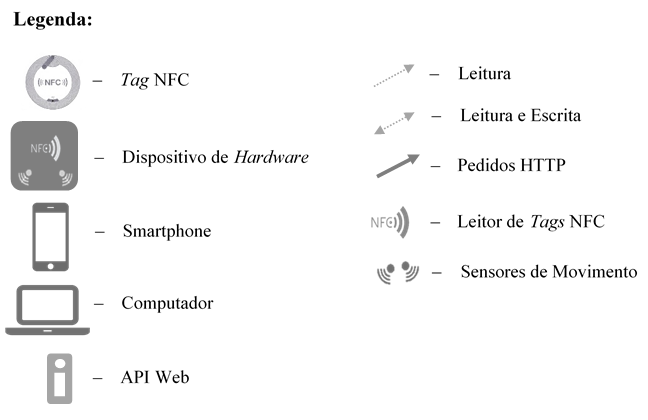
\includegraphics[width=12cm, scale=1]{./figures/project_structures_caption.png}
\end{center}

Com a Figura \ref{project-structure} pretende-se não só apresentar os principais componentes do projeto, bem como demonstrar de forma breve a relação dos mesmos. É de destacar que uma \textit{tag} pode ser lida por um dispositivo de \textit{hardware} munido de um leitor de \textit{tags}. Um \textit{smartphone} equipado com tecnologia \acrshort{nfc} pode escrever na \textit{tag} \acrshort{nfc}, tal é necessário para identificar produtos avulsos presentes num sistema de arrumação. Tanto o dispositivo de \textit{hardware} como as aplicações, móvel e \textit{web}, comunicam com a \gls{api-web}.\\

O projeto é composto por 2 blocos principais, que se relacionam. A Figura \ref{project-architecture} representa esses blocos. 

\begin{figure}[H]
	\centering
	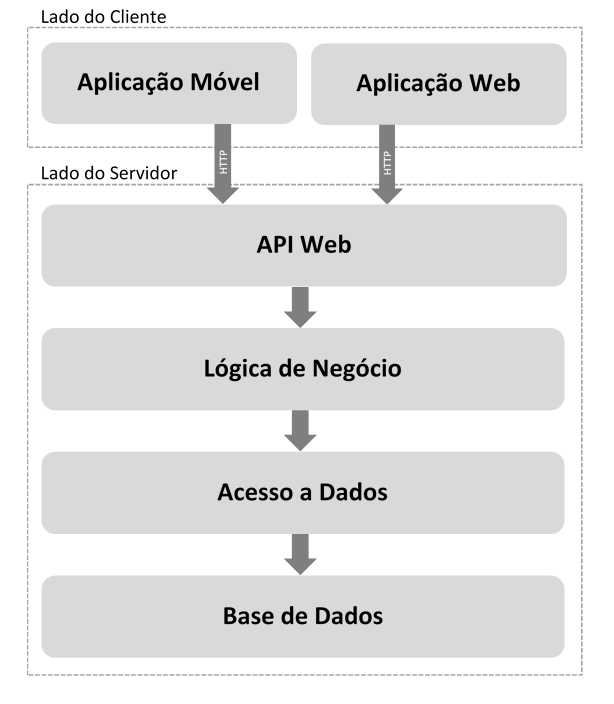
\includegraphics[height=9cm, scale=1]{./figures/project_architecture.png}
	\caption{Arquitetura do Projeto}
	\label{project-architecture}
\end{figure}

O lado do servidor incluí quatro camadas e expõe uma \gls{api-web}. A camada da \acrfull{bd} é realizada com o \acrfull{sgbd} \textit{PostgreSQL}. A \acrfull{dal} é responsável pelas leituras e escritas à \acrshort{bd}. Esta camada é produzida com a linguagem de programação \textit{Java}, com a \acrfull{jpa}. A \acrfull{bll} é responsável pela gestão dos dados obtidos da \acrshort{bd} ou dos \textit{controllers}. A implementação desta camada recorreu à mesma ferramenta que foi usada na \acrshort{dal}. Os \textit{controllers} foram desenvolvidos em \textit{Java} com a \textit{framework} da \textit{Spring}, chamada de \textit{Spring Boot}. A \gls{api-web} disponibiliza recursos em diferentes \textit{hypermedia}.

Do lado do cliente existem dois modos de interação, por uma aplicação móvel e outra por uma aplicação web. A aplicação móvel disponível para a plataforma \textit{Android}, desenvolvida em linguagem \textit{Kotlin}. A aplicação web é disponibilizada para a maioria dos browsers, implementada utilizando a linguagem \textit{JavaScript}, com o auxilio da \textit{framework Express}.


%
% Secção 1.4
%
\section{Estrutura do Relatório} \label{sec14}
O relatório está estruturado em 4 capítulos.

O capítulo 2 formula o problema, detalhando os requisitos do projeto. São ainda apresentadas as dificuldades encontradas ao longo do projeto. 

No capítulo 3 o problema é solucionado, sendo apresentada, com detalhe, a solução implementada. O capítulo foi dividido pelas várias camadas que compõe o projeto. Na secção \ref{sec31} expõe-se a modelagem dada aos dados. Por conseguinte, a secção \ref{sec32} explicita de que forma esses dados foram armazenados, sendo ainda justificadas as decisões tomadas nesta camada. A secção \ref{sec33} fundamenta a seleção das ferramentas utilizadas para a implementação. A lógica de negócio está presente na secção \ref{sec34}. 

É no capítulo 4 que se retiram conclusões face ao trabalho desenvolvido em relação ao trabalho inicialmente previsto. Este planeamento inicial é revelado na secção \ref{sec41}. Para finalizar, propõe-se o trabalho a realizar futuramente, na secção \ref{sec43}.

No Anexo A define-se terminologia, quer a básica à gestão de stocks, para melhor compreensão de alguns dos termos utilizados no decorrer do projeto, quer de conceitos de programação.
